\documentclass[UTF8, a4paper]{ctexart}
\usepackage[margin=2.5cm]{geometry}
\usepackage{fontspec}
\setmainfont{Times New Roman}
\usepackage{amsmath, amssymb, amsfonts, mathtools}
\usepackage{tikz}
\usetikzlibrary{shapes.geometric, arrows.meta, positioning, calc, fit, backgrounds, decorations.pathreplacing}
\usepackage{graphicx}
\usepackage{booktabs}
\usepackage{xcolor}
\usepackage{listings}
\usepackage{hyperref}
\usepackage{enumitem}
\usepackage{caption}
\usepackage{float}
\usepackage{array}
\usepackage{multirow}
\usepackage{fancyhdr}
\usepackage{titlesec}

% 页面样式
\pagestyle{fancy}
\fancyhf{}
\fancyhead[L]{\small $\mu$-MuZero 项目学习手册}
\fancyhead[R]{\small \leftmark}
\fancyfoot[C]{\thepage}
\renewcommand{\headrulewidth}{0.4pt}

% 章节样式
\titleformat{\section}{\Large\bfseries\color{blue!70!black}}{\thesection}{1em}{}
\titleformat{\subsection}{\large\bfseries\color{blue!50!black}}{\thesubsection}{1em}{}

% 代码样式
\lstset{
    language=Python,
    basicstyle=\ttfamily\small,
    keywordstyle=\color{blue!70!black}\bfseries,
    commentstyle=\color{green!50!black},
    stringstyle=\color{orange!80!black},
    numbers=left,
    numberstyle=\tiny\color{gray},
    frame=single,
    breaklines=true,
    backgroundcolor=\color{gray!5},
    showstringspaces=false,
    tabsize=4,
    xleftmargin=2em,
    framexleftmargin=1.5em
}

% 自定义颜色
\definecolor{netcolor}{RGB}{70,130,180}
\definecolor{envcolor}{RGB}{60,150,100}
\definecolor{mctscolor}{RGB}{180,100,60}
\definecolor{traincolor}{RGB}{140,80,160}

\begin{document}

% ==================== 封面 ====================
\begin{titlepage}
\centering
\vspace*{3cm}
{\Huge\bfseries $\mu$-MuZero 项目完整学习手册\\[0.8cm]}
{\Large 面向自主微机器人手术的模型强化学习\\[0.3cm]}
{\large 安全约束随机变体的深度解析\\[2cm]}

\begin{tikzpicture}[
    box/.style={rectangle, rounded corners, draw, minimum width=2.5cm, minimum height=1cm, align=center, font=\small},
    arrow/.style={-{Stealth[length=2mm]}, thick}
]
\node[box, fill=blue!15] (obs) at (0,0) {观测图像};
\node[box, fill=netcolor!20] (rep) at (3.5,0) {表征网络 $h_\theta$};
\node[box, fill=mctscolor!20] (mcts) at (7.5,0) {安全约束 MCTS};
\node[box, fill=traincolor!20] (act) at (11,0) {动作 $(t,p)$};
\node[box, fill=envcolor!20] (env) at (11,-2.5) {数字孪生环境};

\draw[arrow] (obs) -- (rep);
\draw[arrow] (rep) -- (mcts);
\draw[arrow] (mcts) -- (act);
\draw[arrow] (act) -- (env);
\draw[arrow, dashed] (env.west) -- ++(-2,0) |- (obs.west);
\end{tikzpicture}

\vfill
{\large 作者：Yunxiao Ren\\[0.2cm]}
{\large 帝国理工学院 哈姆林机器人手术中心\\[0.5cm]}
{\large \today\\[1cm]}
\end{titlepage}

% ==================== 目录 ====================
\tableofcontents
\newpage

% ==================== 第1章 ====================
\section{项目概述与背景}

\subsection{什么是 $\mu$-MuZero？}

\textbf{$\mu$-MuZero}（micro-MuZero）是一种专门为\textbf{自主光学微操作}设计的模型强化学习算法，应用于微创外科手术场景。

在细胞级别的手术中，光学微机器人可以利用激光光阱（Optical Tweezers）实现亚微米精度的操控，但目前这些系统仍然依赖\textbf{手动操作}。人类反应时间约为 250 ms，对于微尺度流体动力学而言太慢了。因此，需要自主的强化学习代理来实时决策。

\subsection{微尺度带来的三大挑战}

现有 RL 算法在宏观尺度表现良好，但在微尺度面临根本性的不同问题：

\begin{table}[H]
\centering
\caption{宏观尺度 vs 微尺度强化学习的差异}
\begin{tabular}{@{}lll@{}}
\toprule
\textbf{挑战维度} & \textbf{宏观 RL} & \textbf{微尺度 RL} \\
\midrule
动力学特性 & 确定性（惯性主导） & \textbf{随机性}（布朗运动主导） \\
安全性要求 & 软偏好 & \textbf{硬约束}（激光功率上限、光毒性） \\
动作空间 & 离散/连续 & \textbf{组合爆炸}（$K$ 光阱 $\times$ 7 原语 $= 7^K$ 种动作） \\
\bottomrule
\end{tabular}
\end{table}

\subsection{$\mu$-MuZero 的核心解决方案}

针对上述三个挑战，$\mu$-MuZero 提出了三项核心创新：

\begin{enumerate}[leftmargin=2em]
    \item \textbf{随机潜态动力学}：显式建模高斯不确定性，$s' \sim \mathcal{N}(\mu_\theta(s,a), \sigma_\theta(s,a))$
    \item \textbf{安全约束 MCTS}：在规划阶段硬剪枝危险动作
    \item \textbf{分解动作表示}：将 ``选哪个光阱'' 与 ``如何移动'' 解耦
\end{enumerate}

\subsection{性能基准}

在基于数字孪生的仿真验证中，$\mu$-MuZero 取得了显著优于基线方法的性能：

\begin{table}[H]
\centering
\caption{各任务成功率对比（\%）}
\begin{tabular}{@{}lccccc@{}}
\toprule
\textbf{任务} & \textbf{$\mu$-MuZero} & \textbf{脚本法} & \textbf{PPO} & \textbf{人工} & \textbf{Oracle MPC} \\
\midrule
单机器人运输 & \textbf{91.3} & 67.2 & 54.8 & 78.0 & 94.1 \\
避障导航 & \textbf{89.0} & 58.0 & --- & 62.0 & --- \\
协作运输 & \textbf{78.4} & 0 & --- & 34.0 & 85.7 \\
微装配 & \textbf{68.0} & 0 & --- & 8.0 & --- \\
\bottomrule
\end{tabular}
\end{table}

光毒性预算使用率：$\mu$-MuZero \textbf{45\%} vs 人工 68\% vs 脚本 82\%。

\newpage
% ==================== 第2章 ====================
\section{系统整体架构}

\subsection{数据流总览}

$\mu$-MuZero 的完整系统由五个核心模块组成，数据流如下：

\begin{figure}[H]
\centering
\begin{tikzpicture}[
    node distance=1.2cm and 2cm,
    box/.style={rectangle, rounded corners=3pt, draw, thick, minimum width=2.8cm, minimum height=1.2cm, align=center, font=\small\bfseries},
    smallbox/.style={rectangle, rounded corners=2pt, draw, minimum width=2.2cm, minimum height=0.8cm, align=center, font=\scriptsize},
    arrow/.style={-{Stealth[length=2.5mm]}, thick, >=stealth},
    dasharrow/.style={-{Stealth[length=2mm]}, thick, dashed, >=stealth},
]

\node[box, fill=envcolor!15] (env) {数字孪生环境};
\node[box, fill=blue!10, right=of env] (obs) {观测 $o_t$};
\node[box, fill=netcolor!15, above right=0.8cm and 1.5cm of obs] (rep) {表征网络 $h_\theta$};
\node[box, fill=mctscolor!15, right=2.5cm of rep] (mcts) {安全约束 MCTS};
\node[box, fill=traincolor!15, below right=0.8cm and 1.5cm of mcts] (act) {动作 $a_t$ $(t,p)$};
\node[box, fill=gray!15, below=2.5cm of mcts] (agent) {$\mu$-MuZero Agent};
\node[box, fill=traincolor!10, below=0.8cm of agent] (train) {训练循环};

\draw[arrow] (env) -- node[above, font=\scriptsize] {渲染} (obs);
\draw[arrow] (obs) -- node[above left, font=\scriptsize] {编码} (rep);
\draw[arrow] (rep) -- node[above, font=\scriptsize] {潜态 $s_t$} (mcts);
\draw[arrow] (mcts) -- node[above right, font=\scriptsize] {策略 $\pi$} (act);
\draw[arrow] (act) -- node[right, font=\scriptsize] {执行} (env);
\draw[dasharrow] (agent) -- (rep);
\draw[dasharrow] (agent) -- (mcts);
\draw[dasharrow] (agent) -- (act);
\draw[dasharrow] (train) -- node[left, font=\scriptsize] {梯度更新} (agent);

\end{tikzpicture}
\caption{$\mu$-MuZero 系统数据流图}
\end{figure}

\subsection{模块职责}

\begin{table}[H]
\centering
\caption{各模块职责说明}
\begin{tabular}{@{}lll@{}}
\toprule
\textbf{模块} & \textbf{文件名} & \textbf{核心职责} \\
\midrule
配置模块 & config.py & 集中管理所有超参数与安全约束 \\
神经网络 & networks.py & 表征/动力学/预测三大网络的前向传播 \\
MCTS 规划器 & mcts.py & 安全约束下的蒙特卡洛树搜索 \\
数字孪生 & environment.py & 模拟微尺度物理环境 \\
Agent 接口 & mu\_muzero.py & 整合模型、规划器、环境，实现自博弈 \\
训练脚本 & train.py & 主训练循环、评估、日志记录 \\
PPT 生成器 & ppt\_generator*.py & 自动生成学术演示文稿 \\
\bottomrule
\end{tabular}
\end{table}

\newpage
% ==================== 第3章 ====================
\section{配置模块详解：\texttt{config.py}}

配置模块使用 Python \texttt{dataclass} 实现，集中管理所有超参数，避免分散的魔法数字。

\subsection{配置类定义}

\begin{lstlisting}
from dataclasses import dataclass
from typing import Tuple

@dataclass
class MuMuZeroConfig:
    # 环境参数
    workspace_size: Tuple[float, float, float] = (100.0, 100.0, 50.0)  # um
    num_traps: int = 3
    max_laser_power: float = 100.0  # mW (硬安全约束)
    phototoxicity_budget: float = 5000.0  # mW*ms
    
    # 微物理参数
    viscosity: float = 1.0e-3  # Pa*s (水, 20C)
    temperature: float = 293.15  # K
    brownian_noise_scale: float = 0.1  # um/sqrt(ms)
    
    # 神经网络参数
    latent_dim: int = 256
    num_res_blocks: int = 8
    hidden_dim: int = 256
    
    # MCTS 参数
    num_simulations: int = 50
    c_puct: float = 1.25
    dirichlet_alpha: float = 0.3
    dirichlet_epsilon: float = 0.25
    
    # 训练参数
    batch_size: int = 512
    lr: float = 1e-3
    weight_decay: float = 1e-4
    num_unroll_steps: int = 5
    td_steps: int = 10
\end{lstlisting}

\subsection{参数分类详解}

\subsubsection{环境参数}

\begin{itemize}[leftmargin=2em]
    \item \texttt{workspace\_size = (100, 100, 50)}：三维工作空间（单位：$\mu$m），对应显微镜视野范围。
    \item \texttt{num\_traps = 3}：同时操控的光阱数量，决定动作空间维度。
    \item \texttt{max\_laser\_power = 100.0 mW}：\textbf{硬安全约束}，任何时刻激光功率不得超过此值。
    \item \texttt{phototoxicity\_budget = 5000.0 mW$\cdot$ms}：\textbf{软安全约束}，单回合累积光毒性预算。
\end{itemize}

\subsubsection{微物理参数}

这些参数直接来自流体力学与统计物理：
\begin{itemize}[leftmargin=2em]
    \item \texttt{viscosity = $10^{-3}$ Pa$\cdot$s}：水在 20°C 的动力粘度。
    \item \texttt{temperature = 293.15 K}：绝对温度，用于计算布朗运动强度。
    \item \texttt{brownian\_noise\_scale = 0.1 $\mu$m/$\sqrt{\text{ms}}$}：布朗位移的扩散系数标度。
\end{itemize}

布朗运动的均方位移满足爱因斯坦关系：
\begin{equation}
\langle \Delta x^2 \rangle = 2D\Delta t
\end{equation}
其中扩散系数 $D = \dfrac{k_B T}{6\pi\eta r}$，$k_B$ 为玻尔兹曼常数，$\eta$ 为粘度，$r$ 为粒子半径。

\subsubsection{课程学习阶段}

\begin{lstlisting}
curriculum_stages: Tuple[dict, ...] = (
    {"name": "single_robot", "success_threshold": 0.7, "max_steps": 50000},
    {"name": "obstacle_avoidance", "success_threshold": 0.7, "max_steps": 200000},
    {"name": "two_robot_coop", "success_threshold": 0.7, "max_steps": 800000},
    {"name": "three_robot_assembly", "success_threshold": 0.7, "max_steps": 2000000},
)
\end{lstlisting}

课程学习自动调整任务难度：当最近 100 回合的平均成功率超过 70\% 时，自动进入下一阶段。

\subsubsection{动作原语}

\begin{lstlisting}
trap_primitives: Tuple[str, ...] = ("hold", "N", "S", "E", "W", "up", "down")
\end{lstlisting}

共 7 种原语：保持不动、向北/南/东/西移动（平面 $2\,\mu$m）、向上/下移动（轴向 $1\,\mu$m）。

\newpage
% ==================== 第4章 ====================
\section{神经网络模块详解：\texttt{networks.py}}

神经网络模块是 $\mu$-MuZero 的\textbf{认知核心}，包含三大网络：表征网络 $h_\theta$、动力学网络 $g_\theta$、预测网络 $f_\theta$。

\subsection{整体架构图}

\begin{figure}[H]
\centering
\begin{tikzpicture}[
    node distance=0.8cm and 1.5cm,
    block/.style={rectangle, draw, thick, rounded corners=2pt, minimum width=2.5cm, minimum height=1cm, align=center, font=\small},
    input/.style={rectangle, draw, dashed, thick, minimum width=1.8cm, minimum height=0.7cm, align=center, font=\scriptsize},
    output/.style={rectangle, draw, thick, fill=blue!5, minimum width=1.8cm, minimum height=0.7cm, align=center, font=\scriptsize},
    arrow/.style={-{Stealth[length=2mm]}, thick},
    branch/.style={circle, draw, fill=black, inner sep=1pt}
]

\node[input] (obs) {观测 $o$ (1,224,224)};
\node[block, fill=netcolor!15, right=1.8cm of obs] (conv) {卷积下采样};
\node[block, fill=netcolor!15, right=0.8cm of conv] (res) {残差塔 x8};
\node[block, fill=netcolor!15, right=0.8cm of res] (proj) {全局池化+投影};
\node[input, below=1.8cm of proj] (actvec) {动作编码};
\node[block, fill=mctscolor!15, below left=0.5cm and 0.8cm of actvec] (dynmlp) {MLP (2x)};
\node[block, fill=mctscolor!15, below=0.6cm of dynmlp] (mu) {均值头};
\node[block, fill=mctscolor!15, right=0.6cm of dynmlp] (sigma) {标准差头};
\node[block, fill=mctscolor!15, right=0.6cm of sigma] (rew) {奖励头};
\node[block, fill=traincolor!15, below=2.5cm of proj] (predmlp) {MLP (2x)};
\node[output, below left=0.6cm and 0.3cm of predmlp] (policy) {策略头};
\node[output, below right=0.6cm and 0.3cm of predmlp] (value) {价值头};

\draw[arrow] (obs) -- (conv);
\draw[arrow] (conv) -- (res);
\draw[arrow] (res) -- (proj);
\draw[arrow] (proj) -- node[right, font=\scriptsize] {$s$} ++(0,-1.2) -| (predmlp);
\draw[arrow] (proj) |- ++(0,-0.8) -| (actvec);
\draw[arrow] (actvec) -- (dynmlp);
\draw[arrow] (dynmlp) -- (mu);
\draw[arrow] (dynmlp) -- (sigma);
\draw[arrow] (dynmlp) -- (rew);
\draw[arrow] (predmlp) -- (policy);
\draw[arrow] (predmlp) -- (value);
\node[branch, right=0.3cm of proj] (b1) {};
\draw[arrow] (proj) -- (b1);
\node[above=0.3cm of conv, font=\bfseries] {表征网络 $h_\theta$};
\node[right=0.3cm of rew, font=\bfseries] {动力学网络 $g_\theta$};
\node[below=0.3cm of value, font=\bfseries] {预测网络 $f_\theta$};

\end{tikzpicture}
\caption{$\mu$-MuZero 三大神经网络架构图}
\end{figure}

\subsection{表征网络 $h_\theta$：观测 $\to$ 潜态}

\subsubsection{网络结构}

输入是显微镜灰度图像 $o \in \mathbb{R}^{1 \times 224 \times 224}$，输出是潜态向量 $s \in \mathbb{R}^{256}$。

\begin{lstlisting}
class RepresentationNetwork(nn.Module):
    def __init__(self, in_channels=1, latent_dim=256, num_blocks=8):
        self.conv_init = nn.Sequential(
            nn.Conv2d(1, 64, 3, stride=2, padding=1),   # 112x112
            nn.BatchNorm2d(64), nn.ReLU(),
            nn.Conv2d(64, 128, 3, stride=2, padding=1), # 56x56
            nn.BatchNorm2d(128), nn.ReLU(),
            nn.Conv2d(128, 256, 3, stride=2, padding=1),# 28x28
            nn.BatchNorm2d(256), nn.ReLU(),
        )
        self.res_tower = nn.Sequential(*[
            ResidualBlock(256) for _ in range(8)
        ])
        self.projection = nn.Sequential(
            nn.AdaptiveAvgPool2d(1),  # 1x1
            nn.Flatten(),
            nn.Linear(256, 256), nn.ReLU(),
        )
\end{lstlisting}

\subsubsection{表征网络逐层展开结构}

\begin{figure}[H]
\centering
\begin{tikzpicture}[
    node distance=0.4cm and 0.8cm,
    box/.style={rectangle, draw, thick, rounded corners=2pt, minimum width=1.6cm, minimum height=0.7cm, align=center, font=\scriptsize},
    arrow/.style={-{Stealth[length=1.5mm]}, thick},
    dimlabel/.style={font=\tiny\color{gray}, below=0.05cm}
]
\node[box, fill=blue!10] (in) at (0,0) {输入图像};
\node[box, fill=netcolor!15, right=0.8cm of in] (c1) {Conv (3x3,s=2)};
\node[box, fill=netcolor!15, right=0.6cm of c1] (c2) {Conv (3x3,s=2)};
\node[box, fill=netcolor!15, right=0.6cm of c2] (c3) {Conv (3x3,s=2)};
\node[box, fill=netcolor!20, right=0.8cm of c3, minimum height=1.4cm] (res) {残差塔 x8};
\node[box, fill=netcolor!15, right=0.8cm of res] (gap) {GAP (1x1)};
\node[box, fill=netcolor!15, right=0.6cm of gap] (flat) {Flatten};
\node[box, fill=netcolor!15, right=0.6cm of flat] (proj) {Linear (256)};
\node[box, fill=netcolor!15, right=0.6cm of proj] (relu) {ReLU};
\node[box, fill=blue!15, right=0.8cm of relu] (out) {潜态 $s$};

\node[dimlabel] at (in.south) {$224 \times 224$};
\node[dimlabel] at (c1.south) {$64 \times 112 \times 112$};
\node[dimlabel] at (c2.south) {$128 \times 56 \times 56$};
\node[dimlabel] at (c3.south) {$256 \times 28 \times 28$};
\node[dimlabel] at (res.south) {$256 \times 28 \times 28$};
\node[dimlabel] at (gap.south) {$256 \times 1 \times 1$};
\node[dimlabel] at (flat.south) {$256$};
\node[dimlabel] at (proj.south) {$256$};
\node[dimlabel] at (relu.south) {$256$};
\node[dimlabel] at (out.south) {$256$};

\draw[arrow] (in) -- (c1);
\draw[arrow] (c1) -- (c2);
\draw[arrow] (c2) -- (c3);
\draw[arrow] (c3) -- (res);
\draw[arrow] (res) -- (gap);
\draw[arrow] (gap) -- (flat);
\draw[arrow] (flat) -- (proj);
\draw[arrow] (proj) -- (relu);
\draw[arrow] (relu) -- (out);
\end{tikzpicture}
\caption{表征网络 $h_\theta$ 逐层维度展开图}
\end{figure}

\subsubsection{残差块内部结构}

\begin{figure}[H]
\centering
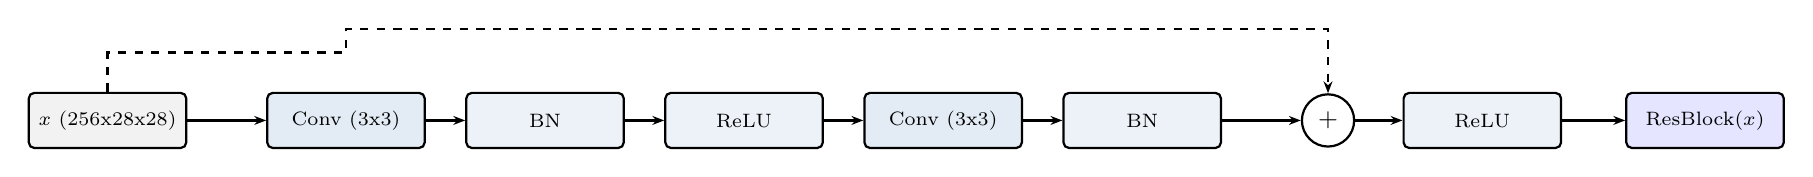
\begin{tikzpicture}[
    node distance=0.6cm and 1.2cm,
    box/.style={rectangle, draw, thick, rounded corners=2pt, minimum width=2cm, minimum height=0.7cm, align=center, font=\scriptsize},
    arrow/.style={-{Stealth[length=1.5mm]}, thick},
    sum/.style={circle, draw, thick, minimum size=0.6cm, align=center, font=\small},
    skip/.style={-{Stealth[length=1.5mm]}, thick, dashed}
]
\node[box, fill=gray!10] (xin) at (0,0) {$x$ (256x28x28)};
\node[box, fill=netcolor!15, right=1cm of xin] (c1) {Conv (3x3)};
\node[box, fill=netcolor!10, right=0.5cm of c1] (bn1) {BN};
\node[box, fill=netcolor!10, right=0.5cm of bn1] (r1) {ReLU};
\node[box, fill=netcolor!15, right=0.5cm of r1] (c2) {Conv (3x3)};
\node[box, fill=netcolor!10, right=0.5cm of c2] (bn2) {BN};
\node[sum, right=1cm of bn2] (sum) {$+$};
\node[box, fill=netcolor!10, right=0.6cm of sum] (relu) {ReLU};
\node[box, fill=blue!10, right=0.8cm of relu] (xout) {ResBlock($x$)};

\node[coordinate, above=0.8cm of c1] (mid) {};
\draw[skip] (xin.north) -- ++(0,0.5) -| (mid) -| (sum.north);
\draw[arrow] (xin) -- (c1);
\draw[arrow] (c1) -- (bn1);
\draw[arrow] (bn1) -- (r1);
\draw[arrow] (r1) -- (c2);
\draw[arrow] (c2) -- (bn2);
\draw[arrow] (bn2) -- (sum);
\draw[arrow] (sum) -- (relu);
\draw[arrow] (relu) -- (xout);
\end{tikzpicture}
\caption{残差块 ResBlock(256) 内部结构}
\end{figure}

\subsubsection{残差块设计}

\begin{equation}
\text{ResBlock}(x) = \text{ReLU}\Big(\text{BN}_2\big(\text{Conv}_2(\text{ReLU}(\text{BN}_1(\text{Conv}_1(x))))\big) + x\Big)
\end{equation}

残差连接缓解梯度消失，使得 8 层残差塔可以稳定训练。

\subsubsection{前向传播公式}

设输入图像为 $o$，则潜态计算为：
\begin{align}
x_0 &= \text{ConvInit}(o) \in \mathbb{R}^{256 \times 28 \times 28} \\
x_1 &= \text{ResTower}(x_0) \\
s &= \text{Projection}(x_1) = \text{ReLU}\big(W_p \cdot \text{GAP}(x_1) + b_p\big) \in \mathbb{R}^{256}
\end{align}

\subsection{动力学网络 $g_\theta$：核心创新}

\subsubsection{为什么需要随机动力学？}

在微尺度低雷诺数环境中，布朗运动不可忽略。50 ms 控制周期内的布朗位移约为：
\begin{equation}
\Delta x_{\text{Brownian}} \approx \sqrt{2D\Delta t} \approx 100\,\text{nm}
\end{equation}
这与光阱的主动位移（$2\,\mu\text{m} = 2000\,\text{nm}$）处于同一数量级，因此不能将环境视为确定性系统。

标准 MuZero 假设：$s_{t+1} = g_\theta(s_t, a_t)$（确定性）

$\mu$-MuZero 假设：
\begin{equation}
\boxed{s_{t+1} \sim \mathcal{N}\big(\mu_\theta(s_t, a_t), \, \sigma_\theta(s_t, a_t)\big)}
\end{equation}

\subsubsection{网络结构}

\begin{lstlisting}
class DynamicsNetwork(nn.Module):
    def __init__(self, latent_dim=256, action_dim=10, reward_support_size=601):
        self.mlp = nn.Sequential(
            nn.Linear(256 + 10, 256), nn.ReLU(),
            nn.Linear(256, 256), nn.ReLU(),
        )
        self.next_state_mu = nn.Linear(256, 256)
        self.next_state_logsigma = nn.Linear(256, 256)
        self.reward_head = nn.Linear(256, 601)
        self.state_norm = nn.BatchNorm1d(256, affine=False)
\end{lstlisting}

\subsubsection{动力学网络详细结构}

\begin{figure}[H]
\centering
\begin{tikzpicture}[
    node distance=0.5cm and 0.8cm,
    box/.style={rectangle, draw, thick, rounded corners=2pt, minimum width=1.8cm, minimum height=0.7cm, align=center, font=\scriptsize},
    arrow/.style={-{Stealth[length=1.5mm]}, thick},
    concat/.style={rectangle, draw, thick, dashed, minimum width=0.8cm, minimum height=0.6cm, align=center, font=\scriptsize},
    dimlabel/.style={font=\tiny\color{gray}, below=0.05cm}
]
\node[box, fill=blue!10] (s) at (0,0) {潜态 $s_t$};
\node[box, fill=traincolor!10] (a) at (0,-1.3) {动作 $a_t$};
\node[concat, right=0.6cm of s, yshift=-0.65cm] (cat) {拼接};
\node[box, fill=mctscolor!15, right=0.8cm of cat] (l1) {Linear (266$\to$256)};
\node[box, fill=mctscolor!10, right=0.4cm of l1] (r1) {ReLU};
\node[box, fill=mctscolor!15, right=0.4cm of r1] (l2) {Linear (256$\to$256)};
\node[box, fill=mctscolor!10, right=0.4cm of l2] (r2) {ReLU};
\node[box, fill=orange!15, right=0.8cm of r2, yshift=1.2cm] (mu) {均值头 $\mu_{t+1}$};
\node[box, fill=orange!15, right=0.8cm of r2] (sigma) {标准差头 $\log \sigma_{t+1}$};
\node[box, fill=orange!15, right=0.8cm of r2, yshift=-1.2cm] (reward) {奖励头 $r_{t+1}$};
\node[box, fill=blue!15, right=1cm of mu] (snext) {下一潜态 $s_{t+1}$};
\node[box, fill=mctscolor!10, below=0.3cm of snext, font=\tiny] (sample) {$\mu + \sigma \odot \varepsilon$, BN};

\draw[arrow] (s) -| (cat);
\draw[arrow] (a) -| (cat);
\draw[arrow] (cat) -- node[above, font=\tiny] {$\mathbb{R}^{266}$} (l1);
\draw[arrow] (l1) -- (r1);
\draw[arrow] (r1) -- (l2);
\draw[arrow] (l2) -- (r2);
\draw[arrow] (r2) -- (mu);
\draw[arrow] (r2) -- (sigma);
\draw[arrow] (r2) -- (reward);
\draw[arrow] (mu) -- (snext);
\draw[arrow] (sigma) -| (sample);
\draw[arrow] (sample) -- (snext);
\end{tikzpicture}
\caption{动力学网络 $g_\theta$ 详细结构（含随机采样路径）}
\end{figure}

\subsubsection{前向传播公式}

给定潜态 $s_t \in \mathbb{R}^{256}$ 和动作编码 $a_t \in \mathbb{R}^{K+7}$：
\begin{align}
h_t &= \text{MLP}([s_t; a_t]) \in \mathbb{R}^{256} \\
\mu_{t+1} &= W_\mu h_t + b_\mu \in \mathbb{R}^{256} \\
\log\sigma_{t+1} &= \text{clip}(W_\sigma h_t + b_\sigma, -10, 2) \in \mathbb{R}^{256} \\
r_{t+1} &= W_r h_t + b_r \in \mathbb{R}^{601} \quad \text{(分类分布 logits)}
\end{align}

\texttt{clip} 操作约束标准差范围：$e^{-10} \leq \sigma \leq e^{2}$，避免数值不稳定。

\subsubsection{状态采样}

在推理/规划时，从分布中采样下一状态：
\begin{equation}
s_{t+1} = \mu_{t+1} + \sigma_{t+1} \odot \varepsilon, \quad \varepsilon \sim \mathcal{N}(0, I)
\end{equation}
随后经过状态归一化：$s_{t+1} \leftarrow \text{BatchNorm}(s_{t+1})$。

\subsubsection{奖励分类分布}

与 AlphaZero/MuZero 一致，价值和奖励使用\textbf{分类分布}而非标量回归。支持集为 $[-300, 300]$，步长为 1，共 601 个 bins。

标量值到分类的转换：
\begin{equation}
p_i = \frac{\text{softmax}(z_i)}{\sum_j \text{softmax}(z_j)}, \quad v = \sum_{i=0}^{600} p_i \cdot (i - 300)
\end{equation}

\subsection{预测网络 $f_\theta$：策略与价值估计}

\subsubsection{网络结构}

\begin{lstlisting}
class PredictionNetwork(nn.Module):
    def __init__(self, latent_dim=256, num_actions=21, value_support_size=601):
        self.mlp = nn.Sequential(
            nn.Linear(256, 256), nn.ReLU(),
            nn.Linear(256, 256), nn.ReLU(),
        )
        self.policy_head = nn.Linear(256, 21)
        self.value_head = nn.Linear(256, 601)
\end{lstlisting}

\subsubsection{预测网络详细结构}

\begin{figure}[H]
\centering
\begin{tikzpicture}[
    node distance=0.5cm and 0.8cm,
    box/.style={rectangle, draw, thick, rounded corners=2pt, minimum width=1.8cm, minimum height=0.7cm, align=center, font=\scriptsize},
    arrow/.style={-{Stealth[length=1.5mm]}, thick},
    dimlabel/.style={font=\tiny\color{gray}, below=0.05cm}
]
\node[box, fill=blue!10] (s) at (0,0) {潜态 $s$};
\node[box, fill=traincolor!15, right=0.8cm of s] (l1) {Linear (256$\to$256)};
\node[box, fill=traincolor!10, right=0.4cm of l1] (r1) {ReLU};
\node[box, fill=traincolor!15, right=0.4cm of r1] (l2) {Linear (256$\to$256)};
\node[box, fill=traincolor!10, right=0.4cm of l2] (r2) {ReLU};
\node[box, fill=green!15, right=0.8cm of r2, yshift=0.9cm] (policy) {策略头 $\pi$};
\node[box, fill=green!15, right=0.8cm of r2, yshift=-0.9cm] (value) {价值头 $V$};
\node[box, fill=green!10, right=0.6cm of policy] (sm) {Softmax};
\node[box, fill=green!10, right=0.6cm of value] (scalar) {标量化};
\node[box, fill=blue!15, right=0.6cm of sm] (pout) {策略分布};
\node[box, fill=blue!15, right=0.6cm of scalar] (vout) {价值估计};

\draw[arrow] (s) -- (l1);
\draw[arrow] (l1) -- (r1);
\draw[arrow] (r1) -- (l2);
\draw[arrow] (l2) -- (r2);
\draw[arrow] (r2) -- (policy);
\draw[arrow] (r2) -- (value);
\draw[arrow] (policy) -- (sm);
\draw[arrow] (sm) -- (pout);
\draw[arrow] (value) -- (scalar);
\draw[arrow] (scalar) -- (vout);
\end{tikzpicture}
\caption{预测网络 $f_\theta$ 详细结构（双头输出）}
\end{figure}

\subsubsection{前向传播公式}

\begin{align}
h &= \text{MLP}(s) \in \mathbb{R}^{256} \\
\pi &= \text{softmax}(W_\pi h + b_\pi) \in \Delta^{K\times 7 - 1} \quad \text{(策略分布)} \\
z_v &= W_v h + b_v \in \mathbb{R}^{601} \quad \text{(价值 logits)}
\end{align}

\subsection{分解动作编码}

动作空间被分解为 ``选光阱'' + ``选原语''：
\begin{lstlisting}
def encode_action(self, trap_id, primitive_id):
    trap_onehot = F.one_hot(trap_id, num_classes=K).float()
    prim_onehot = F.one_hot(primitive_id, num_classes=7).float()
    return torch.cat([trap_onehot, prim_onehot], dim=-1)
\end{lstlisting}

动作编码维度为 $K + 7$。总动作数为 $K \times 7$（如 $K=3$ 时为 21）。

\textbf{组合爆炸的解决}：
\begin{itemize}[leftmargin=2em]
    \item 朴素联合动作空间：$7^K$（$K=3$ 时为 343；$K=6$ 时为 117,649）
    \item 分解后动作空间：$K \times 7$（$K=3$ 时为 21；$K=6$ 时为 42）
\end{itemize}

\subsection{整体模型封装}

\texttt{MuMuZeroModel} 将三个网络组合，提供统一接口：

\begin{align}
\text{initial\_inference}(o) &:\quad s_0 = h_\theta(o), \quad (\pi_0, z_0) = f_\theta(s_0) \\
\text{recurrent\_inference}(s, a) &:\quad s' = g_\theta(s, a), \quad r = R_\theta(s, a), \quad (\pi', z') = f_\theta(s')
\end{align}

\subsubsection{完整推理流程对比}

\begin{figure}[H]
\centering
\begin{tikzpicture}[
    node distance=0.4cm and 0.6cm,
    box/.style={rectangle, draw, thick, rounded corners=2pt, minimum width=1.6cm, minimum height=0.6cm, align=center, font=\scriptsize},
    arrow/.style={-{Stealth[length=1.5mm]}, thick},
    dasharrow/.style={-{Stealth[length=1.5mm]}, thick, dashed},
    bigbox/.style={rectangle, draw, thick, dashed, rounded corners=3pt, inner sep=0.3cm}
]
\node[font=\bfseries\small] (initlabel) at (-2, 0.8) {初始推理};
\node[box, fill=blue!10] (obs) at (0,0) {观测 $o$};
\node[box, fill=netcolor!15, right=0.8cm of obs] (h) {$h_\theta$};
\node[box, fill=blue!15, right=0.8cm of h] (s0) {潜态 $s_0$};
\node[box, fill=traincolor!15, right=0.8cm of s0] (f) {$f_\theta$};
\node[box, fill=green!15, above right=0.2cm and 0.6cm of f] (pi0) {策略 $\pi_0$};
\node[box, fill=green!15, below right=0.2cm and 0.6cm of f] (v0) {价值 $V_0$};

\draw[arrow] (obs) -- (h);
\draw[arrow] (h) -- (s0);
\draw[arrow] (s0) -- (f);
\draw[arrow] (f) -- (pi0);
\draw[arrow] (f) -- (v0);

\begin{scope}[on background layer]
\node[bigbox, fill=gray!5, fit=(obs)(h)(s0)(f)(pi0)(v0)(initlabel)] (initbox) {};
\end{scope}

\node[font=\bfseries\small] (reclabel) at (-2, -3.2) {循环推理};
\node[box, fill=blue!15] (st) at (0,-4) {潜态 $s_t$};
\node[box, fill=traincolor!10, below=0.5cm of st] (at) {动作 $a_t$};
\node[box, fill=mctscolor!15, right=0.8cm of st, yshift=-0.25cm] (g) {$g_\theta$};
\node[box, fill=blue!15, right=0.8cm of g] (st1) {潜态 $s_{t+1}$};
\node[box, fill=orange!15, below=0.4cm of st1] (rt1) {奖励 $r_{t+1}$};
\node[box, fill=traincolor!15, right=0.8cm of st1] (f2) {$f_\theta$};
\node[box, fill=green!15, above right=0.2cm and 0.6cm of f2] (pi1) {策略 $\pi_{t+1}$};
\node[box, fill=green!15, below right=0.2cm and 0.6cm of f2] (v1) {价值 $V_{t+1}$};

\draw[arrow] (st) -| (g);
\draw[arrow] (at) -| (g);
\draw[arrow] (g) -- (st1);
\draw[arrow] (g) -- (rt1);
\draw[arrow] (st1) -- (f2);
\draw[arrow] (f2) -- (pi1);
\draw[arrow] (f2) -- (v1);

\begin{scope}[on background layer]
\node[bigbox, fill=gray!5, fit=(st)(at)(g)(st1)(rt1)(f2)(pi1)(v1)(reclabel)] (recbox) {};
\end{scope}

\draw[dasharrow] (s0.south) -- ++(0,-0.8) -| (st.north) node[midway, right, font=\tiny] {MCTS展开};

\end{tikzpicture}
\caption{初始推理 vs 循环推理对比图}
\end{figure}

\newpage
% ==================== 第5章 ====================
\section{环境模块详解：\texttt{environment.py}}

数字孪生环境模拟了光学微操作中的完整物理过程，是代理训练的\textbf{仿真沙盒}。

\subsection{物理模型组成}

\begin{figure}[H]
\centering
\begin{tikzpicture}[
    box/.style={rectangle, rounded corners, draw, thick, minimum width=2.8cm, minimum height=1cm, align=center, font=\small},
    arrow/.style={-{Stealth[length=2mm]}, thick}
]
\node[box, fill=blue!10] (img) at (0,0) {显微镜图像};
\node[box, fill=netcolor!15] (force) at (4,0) {光力模型};
\node[box, fill=envcolor!15] (hydro) at (8,0) {流体动力学};
\node[box, fill=mctscolor!15] (brown) at (8,-2) {布朗运动};
\node[box, fill=traincolor!15] (dyn) at (4,-2) {过阻尼动力学};

\draw[arrow] (force) -- (dyn) node[midway, right, font=\scriptsize] {$F_{\text{optical}}$};
\draw[arrow] (hydro) -- (dyn) node[midway, above, font=\scriptsize] {$\gamma$};
\draw[arrow] (brown) -- (dyn) node[midway, right, font=\scriptsize] {$F_B$};
\draw[arrow] (dyn) -- (img) node[midway, left, font=\scriptsize] {位置};
\end{tikzpicture}
\caption{数字孪生物理模型组成}
\end{figure}

\subsection{光力模型：\texttt{LearnedForceModel}}

光学力场高度非线性，无闭式解。使用神经网络近似：

\subsubsection{网络结构}

\begin{lstlisting}
class LearnedForceModel(nn.Module):
    def __init__(self, input_dim=6, hidden_dim=128):
        self.B = nn.Parameter(torch.randn(3, 32) * 2.0, requires_grad=False)
        self.net = nn.Sequential(
            nn.Linear(input_dim, 128), nn.ReLU(),
            nn.Linear(128, 128), nn.ReLU(),
            nn.Linear(128, 128), nn.ReLU(),
            nn.Linear(128, 3),  # 3D 力 (pN)
        )
\end{lstlisting}

\subsubsection{傅里叶特征嵌入}

为捕捉高频变化的光力场，对相对位置使用随机傅里叶特征：
\begin{equation}
\phi(x) = \begin{bmatrix} \sin(2\pi x B) \\ \cos(2\pi x B) \end{bmatrix} \in \mathbb{R}^{64}
\end{equation}
其中 $B \in \mathbb{R}^{3 \times 32}$ 为随机采样矩阵，$B_{ij} \sim \mathcal{N}(0, 4)$。

\subsubsection{前向传播}

输入：光阱-机器人相对位置 $x_{\text{rel}} \in \mathbb{R}^3$，机器人朝向 $\theta \in \mathbb{R}^3$。

\begin{equation}
F_{\text{optical}} = \text{MLP}\big([\phi(x_{\text{rel}}); \theta]\big) \in \mathbb{R}^3 \quad \text{(单位：pN)}
\end{equation}

\subsection{过阻尼动力学}

在微尺度（低雷诺数 $Re \ll 1$），惯性项可忽略，运动由力平衡主导：

\subsubsection{Stokes 阻力}

半径为 $r$ 的球体在粘度为 $\eta$ 的流体中的阻力系数：
\begin{equation}
\boxed{\gamma = 6\pi\eta r}
\end{equation}

对于 $r = 2\,\mu\text{m}$ 的机器人，在水中（$\eta = 10^{-3}\,\text{Pa}\cdot\text{s}$）：
\begin{equation}
\gamma = 6\pi \times 10^{-3} \times 2\times 10^{-6} \approx 3.77 \times 10^{-8}\,\text{N}\cdot\text{s}/\text{m}
\end{equation}

\subsubsection{布朗力}

由涨落耗散定理，布朗力满足：
\begin{equation}
\langle F_B(t) \rangle = 0, \quad \langle F_B(t) F_B(t') \rangle = 2\gamma k_B T \delta(t - t')
\end{equation}

离散形式（Euler-Maruyama）：
\begin{equation}
F_B \sim \mathcal{N}\Big(0, \, \frac{2\gamma k_B T}{\Delta t}\Big)
\end{equation}

代码中简化为尺度参数化的位置域噪声：
\begin{equation}
\Delta x_B \sim \mathcal{N}(0, \sigma_B^2), \quad \sigma_B = 0.1\,\mu\text{m}/\sqrt{\text{ms}}
\end{equation}

\subsubsection{速度-位置更新}

力平衡方程 $\gamma v = F_{\text{optical}} + F_B$ 解得：
\begin{equation}
\boxed{v = \frac{F_{\text{optical}} + F_B}{\gamma} \times 10^6 \quad [\mu\text{m}/\text{s}]}
\end{equation}
位置更新：
\begin{equation}
x_{t+1} = x_t + v \cdot \Delta t, \quad \Delta t = 50\,\text{ms}
\end{equation}

\subsection{观测生成}

环境生成简化的 224$\times$224 灰度显微镜图像：

\begin{lstlisting}
def _get_observation(self):
    img = np.zeros((224, 224))
    scale = 224.0 / 100.0  # 100 um -> 224 px
    
    for robot in self.robots:
        x, y = int(robot['pos'][0] * scale), int(robot['pos'][1] * scale)
        # 高斯点扩散函数 (PSF)
        blob = exp(-((xx - x)**2 + (yy - y)**2) / (2 * sigma^2))
        img += blob * 0.8
    
    # 添加传感器噪声
    img += np.random.normal(0, 0.05, img.shape)
    img = np.clip(img, 0, 1)
\end{lstlisting}

机器人渲染为 $\sigma = 3$ 像素的高斯 blob，目标细胞为 $\sigma = 8$ 像素。

\subsection{奖励函数设计}

\begin{equation}
\boxed{R_t = -0.1 \cdot d_{\text{goal}} - 0.01 \cdot t - 10.0 \cdot \mathbf{1}_{[PT > B]} + 10.0 \cdot \mathbf{1}_{[d_{\text{goal}} < 2\mu\text{m}]}}
\end{equation}

其中：
\begin{itemize}[leftmargin=2em]
    \item $d_{\text{goal}}$：目标到目标位置的距离（$\mu$m）
    \item $t$：当前步数（效率惩罚）
    \item $PT$：累积光毒性（mW$\cdot$ms）
    \item $B$：光毒性预算 5000 mW$\cdot$ms
\end{itemize}

\subsection{终止条件}

\begin{equation}
\text{done} = \mathbf{1}_{[d_{\text{goal}} < 2\mu\text{m}]} \;\lor\; \mathbf{1}_{[PT > 1.5B]} \;\lor\; \mathbf{1}_{[t > 500]}
\end{equation}

\newpage
% ==================== 第6章 ====================
\section{MCTS 模块详解：\texttt{mcts.py}}

蒙特卡洛树搜索是 $\mu$-MuZero 的\textbf{决策引擎}。在标准 MuZero MCTS 基础上，增加了安全约束和不确定性感知。

\subsection{标准 MuZero MCTS 回顾}

MuZero 的 MCTS 包含四个阶段：
\begin{enumerate}[leftmargin=2em]
    \item \textbf{SELECT}：从根节点选择子节点，直到到达叶节点
    \item \textbf{EXPAND}：展开叶节点，用预测网络生成先验概率
    \item \textbf{EVALUATE}：评估叶节点价值
    \item \textbf{BACKPROPAGATE}：将价值反向传播到根路径
\end{enumerate}

\subsection{$\mu$-MuZero MCTS 改进流程图}

\begin{figure}[H]
\centering
\begin{tikzpicture}[
    node distance=0.6cm and 1.2cm,
    block/.style={rectangle, draw, thick, rounded corners=2pt, minimum width=2.5cm, minimum height=0.9cm, align=center, font=\small},
    decision/.style={diamond, draw, thick, aspect=2, minimum width=1.5cm, minimum height=0.8cm, align=center, font=\scriptsize},
    arrow/.style={-{Stealth[length=2mm]}, thick}
]
\node[block, fill=gray!10] (root) at (0,0) {初始化根节点};
\node[block, fill=blue!10] (expand) at (0,-1.5) {展开根节点};
\node[block, fill=green!10] (noise) at (0,-3) {Dirichlet 噪声};
\node[block, fill=yellow!10] (sim) at (0,-4.5) {单次模拟};
\node[block, fill=cyan!10] (select) at (-3,-4.5) {SELECT};
\node[block, fill=orange!10] (safety) at (-3,-6) {SAFETY 剪枝};
\node[block, fill=red!10] (sample) at (0,-6) {SAMPLE 采样};
\node[block, fill=purple!10] (back) at (3,-6) {BACKPROP};
\node[block, fill=gray!10] (done) at (0,-7.5) {返回访问计数};

\draw[arrow] (root) -- (expand);
\draw[arrow] (expand) -- (noise);
\draw[arrow] (noise) -- (sim);
\draw[arrow] (sim) -- (select);
\draw[arrow] (select) -- (safety);
\draw[arrow] (safety) -- (sample);
\draw[arrow] (sample) -- (back);
\draw[arrow] (back) -- (0,-6) -- (0,-4.5);
\draw[arrow] (sim) -- (done) node[midway, right, font=\scriptsize] {重复 $N_{\text{sim}}$ 次};
\end{tikzpicture}
\caption{安全约束 MCTS 流程图}
\end{figure}

\subsection{节点数据结构}

\begin{lstlisting}
class Node:
    def __init__(self, prior):
        self.prior = prior        # 先验概率 P(a)
        self.visit_count = 0      # 访问次数 N(a)
        self.value_sum = 0.0      # 累积价值 W(a)
        self.children = {}        # 子节点字典
        self.hidden_state = None  # 潜态 s
        self.reward = 0.0         # 即时奖励 r
        self.is_safe = True       # 安全标志（新增）
\end{lstlisting}

节点价值：$Q(a) = \dfrac{W(a)}{N(a)}$（若 $N(a) > 0$，否则 $Q(a) = 0$）。

\subsection{UCB 选择与不确定性惩罚}

\subsubsection{标准 UCB 公式}

在标准 MuZero 中，子节点选择标准为：
\begin{equation}
\text{UCB}(s, a) = Q(s, a) + c_{\text{puct}} \cdot P(a) \cdot \frac{\sqrt{N(s)}}{1 + N(s, a)}
\end{equation}

\subsubsection{$\mu$-MuZero 改进公式}

引入不确定性惩罚项 $\lambda_U$：
\begin{equation}
\boxed{\text{UCB}_\mu(s, a) = Q(s, a) + c_{\text{puct}} \cdot P(a) \cdot \frac{\sqrt{N(s)}}{1 + N(s, a)} \cdot \lambda_U}
\end{equation}

其中不确定性惩罚系数：
\begin{equation}
\lambda_U = \frac{1}{1 + w_U \cdot U}, \quad w_U = 0.5
\end{equation}

$U$ 为根节点的不确定性估计（如潜态标准差均值）。$\lambda_U \in (0, 1]$，不确定性越高，探索奖励越小。

\textbf{物理意义}：当代理对环境状态不确定时（如图像模糊、目标丢失），应减少冒险的探索行为，选择更保守的动作。

\subsection{安全剪枝机制}

\subsubsection{三级安全约束}

\begin{table}[H]
\centering
\caption{安全约束层级}
\begin{tabular}{@{}cll@{}}
\toprule
\textbf{层级} & \textbf{类型} & \textbf{实现方式} \\
\midrule
Level 1 & 硬约束 & MCTS 直接剪枝危险动作 \\
Level 2 & 软约束 & 奖励函数中惩罚光毒性超支 \\
Level 3 & 认知约束 & 高不确定性降低探索奖励 \\
\bottomrule
\end{tabular}
\end{table}

\subsubsection{硬剪枝实现}

\begin{lstlisting}
def _check_action_safety(self, action_idx, latent):
    trap_id, prim_id = self.action_map[action_idx]
    primitive = self.config.trap_primitives[prim_id]
    
    # 禁止显式增加激光功率
    if primitive == "incr_power":
        return False
    
    # 边界移动理论上由 MPC 处理
    if primitive in ("N", "S", "E", "W", "up", "down"):
        return True
    
    return True
\end{lstlisting}

注意：当前实现较为简化。在完整系统中，应从潜态解码当前位置，精确计算移动后的边界碰撞和功率变化。

\subsubsection{状态安全验证}

展开新节点前，检查状态安全性：
\begin{lstlisting}
def _is_safe_state(self, latent, action):
    _, value_logits = self.model.prediction(latent)
    value = scalar_from_support(value_logits)
    return value > -10.0  # 启发式阈值
\end{lstlisting}

使用价值估计作为安全代理：若某状态的价值低于阈值，认为该状态危险，不再展开。

\subsection{Dirichlet 噪声（根节点探索）}

为根节点先验添加 Dirichlet 噪声，防止过早收敛到次优动作：
\begin{equation}
\tilde{P}(a) = (1 - \varepsilon) P(a) + \varepsilon \cdot \eta(a), \quad \eta \sim \text{Dir}(\alpha)
\end{equation}

参数：$\alpha = 0.3$，$\varepsilon = 0.25$。仅对安全动作添加噪声。

\subsection{反向传播}

价值从叶节点回传至根节点：
\begin{equation}
\boxed{V_{\text{backup}} = r + \gamma \cdot V_{\text{child}}, \quad \gamma = 0.997}
\end{equation}

$\mu$-MuZero 增加了不确定性惩罚：
\begin{equation}
V_{\text{backup}}^{(t)} = r_t + \gamma \cdot V_{\text{backup}}^{(t+1)} - 0.1 \cdot U_{\text{root}}
\end{equation}

每经过一个节点，累积价值更新为：
\begin{equation}
W(s, a) \leftarrow W(s, a) + V_{\text{backup}}^{(t)}, \quad N(s, a) \leftarrow N(s, a) + 1
\end{equation}

\subsection{MCTS 输出策略}

模拟结束后，输出为访问计数分布：
\begin{equation}
\pi_{\text{MCTS}}(a) = \frac{N(a)^{1/\tau}}{\sum_{a'} N(a')^{1/\tau}}
\end{equation}

训练时温度 $\tau = 1$（探索），评估时 $\tau \to 0$（贪婪）。

\newpage
% ==================== 第7章 ====================
\section{Agent 模块详解：\texttt{mu\_muzero.py}}

Agent 是系统的\textbf{中央控制器}，将神经网络、MCTS 和环境串联起来，实现完整的自博弈循环。

\subsection{Agent 类结构}

\begin{lstlisting}
class MuMuZeroAgent:
    def __init__(self, config):
        self.device = cuda if available else cpu
        self.model = MuMuZeroModel(config).to(device)
        self.mcts = SafetyConstrainedMCTS(config, self.model)
        self.env = OpticalMicromanipulationEnv(config)
        self.optimizer = Adam(model.parameters(), lr=1e-3, wd=1e-4)
        self.replay_buffer = deque(maxlen=100000)
        self.current_stage = 0  # 课程阶段
\end{lstlisting}

\subsection{动作选择流程}

\begin{figure}[H]
\centering
\begin{tikzpicture}[
    node distance=0.8cm,
    block/.style={rectangle, draw, thick, rounded corners, minimum width=3cm, minimum height=0.8cm, align=center, font=\small},
    arrow/.style={-{Stealth[length=2mm]}, thick}
]
\node[block] (obs) at (0,0) {观测图像 $o_t$};
\node[block, fill=netcolor!15] (rep) at (0,-1.3) {$s_t = h_\theta(o_t)$};
\node[block, fill=mctscolor!15] (mcts) at (0,-2.6) {$\pi_{\text{MCTS}} = \text{MCTS}(s_t)$};
\node[block, fill=traincolor!15] (act) at (0,-3.9) {采样/贪婪选择 $a_t$};
\node[block, fill=envcolor!15] (env) at (0,-5.2) {环境执行，返回 $o_{t+1}, r_t$};

\draw[arrow] (obs) -- (rep);
\draw[arrow] (rep) -- (mcts);
\draw[arrow] (mcts) -- (act);
\draw[arrow] (act) -- (env);
\end{tikzpicture}
\caption{单步决策流程}
\end{figure}

训练时以温度采样选择动作：
\begin{equation}
a_t \sim \text{Cat}(\pi_{\text{MCTS}}) \quad \text{(训练, } \tau = 1\text{)}
\end{equation}

评估时贪婪选择：
\begin{equation}
a_t = \arg\max_a \pi_{\text{MCTS}}(a) \quad \text{(评估, } \tau \to 0\text{)}
\end{equation}

\subsection{动作解码}

将动作索引解码为 (光阱 ID, 原语 ID)：
\begin{equation}
t = \left\lfloor \frac{a}{7} \right\rfloor, \quad p = a \bmod 7
\end{equation}

其中 $t \in \{0, 1, \dots, K-1\}$，$p \in \{0, 1, \dots, 6\}$ 对应 (hold, N, S, E, W, up, down)。

\subsection{回合数据收集}

单回合收集的数据结构：
\begin{equation}
\mathcal{D}_{\text{episode}} = \{(o_t, a_t, \pi_t^{\text{MCTS}}, r_t, V_t)\}_{t=0}^{T}
\end{equation}

其中 $V_t$ 为 n 步折扣回报：
\begin{equation}
\boxed{V_t = \sum_{k=0}^{T-t-1} \gamma^k r_{t+k}}
\end{equation}

代码实现（逆向累积）：
\begin{lstlisting}
def _compute_returns(self, rewards):
    returns = []
    R = 0
    for r in reversed(rewards):
        R = r + 0.997 * R
        returns.insert(0, R)
    return returns
\end{lstlisting}

\subsection{课程学习更新}

\begin{lstlisting}
def update_curriculum(self):
    if len(self.stage_success_history) < 50:
        return
    avg_success = np.mean(self.stage_success_history)
    threshold = self.config.curriculum_stages[self.current_stage]['success_threshold']
    if avg_success > threshold and self.current_stage < 3:
        self.current_stage += 1
        self.stage_success_history.clear()
\end{lstlisting}

课程阶段递进逻辑：
\begin{equation}
\text{stage}_{t+1} = \begin{cases}
\text{stage}_t + 1 & \text{if } \bar{R}_{\text{success}} > 0.7 \text{ and } |\mathcal{H}| \geq 50 \\
\text{stage}_t & \text{otherwise}
\end{cases}
\end{equation}

\newpage
% ==================== 第8章 ====================
\section{训练模块详解：\texttt{train.py}}

训练模块实现了完整的自博弈训练循环，是代理能力成长的\textbf{驱动力}。

\subsection{主训练循环}

\begin{lstlisting}
while step_count < total_steps:
    # 1. 收集自博弈回合
    episode = agent.run_episode(train=True)
    agent.replay_buffer.append(episode)
    
    # 2. 更新课程
    agent.update_curriculum()
    
    # 3. 网络训练
    if len(agent.replay_buffer) >= batch_size:
        batch = random_sample(replay_buffer, batch_size)
        metrics = agent.train_step(batch)
    
    # 4. 日志与保存
    if step_count % log_interval == 0:
        print(f"[Step {step_count}] Loss={metrics['total_loss']:.3f}")
    if step_count % checkpoint_interval == 0:
        agent.save(ckpt_path)
\end{lstlisting}

\subsection{训练步骤：\texttt{train\_step}}

这是最核心的梯度更新函数，包含三个损失项。

\subsubsection{批次采样}

从回放缓冲区采样 $B = 512$ 个回合，每个回合中随机选择一个位置 $k$：
\begin{equation}
k \sim \text{Uniform}\big(0, \, T - K_{\text{unroll}} - 1\big)
\end{equation}

构建训练批次：
\begin{itemize}[leftmargin=2em]
    \item 观测：$o_k$
    \item 目标策略：$\pi_k^{\text{MCTS}}$
    \item 目标价值：$V_k$
    \item 目标奖励序列：$(r_k, r_{k+1}, \dots, r_{k+K-1})$
    \item 动作序列：$(a_k, a_{k+1}, \dots, a_{k+K-1})$
\end{itemize}

\subsubsection{初始推理与策略损失}

\begin{align}
s_0 &= h_\theta(o_k) \\
(\hat{\pi}_0, \hat{z}_0) &= f_\theta(s_0)
\end{align}

策略损失（交叉熵）：
\begin{equation}
\boxed{\mathcal{L}_{\text{policy}} = -\frac{1}{B} \sum_{i=1}^{B} \sum_{a} \pi_k^{(i)}(a) \cdot \log \hat{\pi}_0^{(i)}(a)}
\end{equation}

\subsubsection{价值损失}

将分类分布转换为标量：
\begin{align}
\hat{V}_0 &= \sum_{j=0}^{600} \text{softmax}(\hat{z}_0)_j \cdot (j - 300) \\
\mathcal{L}_{\text{value}} &= \frac{1}{B} \sum_{i=1}^{B} \big(\hat{V}_0^{(i)} - V_k^{(i)}\big)^2
\end{align}

\subsubsection{展开损失（Unroll Loss）}

这是 MuZero 的核心：用学习到的动力学模型展开 $K = 5$ 步，预测中间奖励。

对于第 $m$ 步（$m = 0, 1, \dots, K-1$）：
\begin{align}
s_{m+1} &= g_\theta(s_m, a_{k+m}) \quad \text{（取均值，用于确定性展开）} \\
\hat{r}_{m+1} &= \sum_{j} \text{softmax}(R_{m+1})_j \cdot (j - 300)
\end{align}

奖励损失：
\begin{equation}
\boxed{\mathcal{L}_{\text{reward}} = \frac{1}{K} \sum_{m=0}^{K-1} \frac{1}{B} \sum_{i=1}^{B} \big(\hat{r}_{m+1}^{(i)} - r_{k+m}^{(i)}\big)^2}
\end{equation}

\subsubsection{总损失}

\begin{equation}
\boxed{\mathcal{L}_{\text{total}} = w_\pi \mathcal{L}_{\text{policy}} + w_V \mathcal{L}_{\text{value}} + w_r \mathcal{L}_{\text{reward}}}
\end{equation}

权重配置：$w_\pi = 1.0$，$w_V = 0.25$，$w_r = 1.0$。

价值损失权重较小（0.25）是 MuZero 的标准做法，因为价值估计本身具有较高方差。

\subsubsection{梯度裁剪}

防止梯度爆炸：
\begin{equation}
\|\nabla_\theta \mathcal{L}_{\text{total}}\|_2 \leq 1.0
\end{equation}

\begin{lstlisting}
total_loss.backward()
torch.nn.utils.clip_grad_norm_(model.parameters(), 1.0)
optimizer.step()
\end{lstlisting}

\subsection{训练流程图}

\begin{figure}[H]
\centering
\begin{tikzpicture}[
    node distance=1cm and 1.5cm,
    block/.style={rectangle, draw, thick, rounded corners, minimum width=2.5cm, minimum height=0.9cm, align=center, font=\small},
    arrow/.style={-{Stealth[length=2mm]}, thick}
]
\node[block, fill=gray!10] (buf) at (0,0) {回放缓冲区};
\node[block, fill=blue!10] (sample) at (0,-1.5) {采样批次};
\node[block, fill=netcolor!15] (init) at (-3,-3) {初始推理};
\node[block, fill=mctscolor!15] (unroll) at (0,-3) {展开推理};
\node[block, fill=traincolor!15] (loss) at (3,-3) {计算损失};
\node[block, fill=green!15] (grad) at (3,-4.5) {反向传播};
\node[block, fill=gray!10] (update) at (0,-4.5) {参数更新};

\draw[arrow] (buf) -- (sample);
\draw[arrow] (sample) -| (init);
\draw[arrow] (sample) -- (unroll);
\draw[arrow] (init) -- (loss);
\draw[arrow] (unroll) -- (loss);
\draw[arrow] (loss) -- (grad);
\draw[arrow] (grad) -- (update);
\end{tikzpicture}
\caption{训练步骤数据流}
\end{figure}

\newpage
% ==================== 第9章 ====================
\section{PPT 生成模块}

项目包含两个版本的演示文稿生成器：

\subsection{基础版：\texttt{ppt\_generator.py}}

使用 \texttt{python-pptx} 库生成 13 页学术演示文稿，包含：
\begin{enumerate}[leftmargin=2em]
    \item 标题页
    \item 研究动机
    \item 核心洞察
    \item 算法架构（双栏）
    \item 随机动力学创新
    \item 安全约束创新
    \item 分解动作创新
    \item 课程学习
    \item 应用场景（双栏）
    \item Sim-to-Real 路径
    \item 性能总结
    \item 未来方向
    \item 参考文献
\end{enumerate}

\subsection{增强版：\texttt{ppt\_generator\_v2.py}}

生成双语版本（英文/中文各 14 页），并支持插入公式图片和论文插图。

\begin{lstlisting}
# 生成英文版
build_presentation("en")
# 生成中文版
build_presentation("zh")
# 输出：slides/mu_muzero_algorithm_en.pptx
#       slides/mu_muzero_algorithm_zh.pptx
\end{lstlisting}

\newpage
% ==================== 第10章 ====================
\section{项目总结与学习要点}

\subsection{核心创新回顾}

\begin{table}[H]
\centering
\caption{$\mu$-MuZero 三大创新点}
\begin{tabular}{@{}lp{8cm}@{}}
\toprule
\textbf{创新} & \textbf{核心内容} \\
\midrule
随机潜态动力学 & $s' \sim \mathcal{N}(\mu_\theta, \sigma_\theta)$，显式建模布朗运动不确定性 \\
安全约束 MCTS & 三级安全（硬剪枝/软惩罚/认知折扣），约束违反率降至 0.3\% \\
分解动作表示 & $7^K \to K + 7$，分支因子从 117,649 降至 12（$K=6$） \\
\bottomrule
\end{tabular}
\end{table}

\subsection{关键公式速查}

\begin{align}
\text{随机动力学：} & \quad s_{t+1} = \mu_\theta(s_t, a_t) + \sigma_\theta(s_t, a_t) \odot \varepsilon \\
\text{UCB 选择：} & \quad \text{UCB} = Q + c_{\text{puct}} P \frac{\sqrt{N}}{1+n} \cdot \frac{1}{1 + w_U U} \\
\text{价值回传：} & \quad V = r + \gamma V_{\text{child}} - 0.1 U, \quad \gamma = 0.997 \\
\text{总损失：} & \quad \mathcal{L} = \mathcal{L}_\pi + 0.25 \mathcal{L}_V + \mathcal{L}_r \\
\text{过阻尼速度：} & \quad v = \frac{F_{\text{optical}} + F_B}{\gamma} \times 10^6 \\
\text{奖励函数：} & \quad R = -0.1 d - 0.01 t - 10 \cdot \mathbf{1}_{[PT > B]} + 10 \cdot \mathbf{1}_{[\text{success}]}
\end{align}

\subsection{代码学习建议}

\begin{enumerate}[leftmargin=2em]
    \item \textbf{入门路径}：config.py $\to$ environment.py $\to$ networks.py $\to$ mcts.py $\to$ mu\_muzero.py $\to$ train.py
    \item \textbf{调试技巧}：先在 environment.py 中运行单步交互，确认物理模型合理
    \item \textbf{训练监控}：关注 value\_loss 是否下降，若 stuck 则检查课程学习阈值
    \item \textbf{扩展方向}：
    \begin{itemize}
        \item 将 2D 图像观测升级为 3D + PSF 卷积
        \item 在 \texttt{\_check\_action\_safety} 中实现真正的潜态解码
        \item 添加多智能体通信机制
        \item 实现真实的 sim-to-real 域随机化
    \end{itemize}
\end{enumerate}

\vspace{1cm}
\begin{center}
\rule{0.6\textwidth}{0.5pt}\\[0.5cm]
{\large\itshape ``在微尺度的随机世界中，安全地规划每一步。''}\\[0.3cm]
--- $\mu$-MuZero 设计哲学
\end{center}

\end{document}
